%*******10********20********30********40********50********60********70********80

% For all chapters, use the newdefined chap{} instead of chapter{}
% This will make the text at the top-left of the page be the same as the chapter

\chap{Υλοποίηση Εφαρμογής} \label{c:exper}
%Εξεταζομενο σεναριο

The suitable architecture and frameworks presented previously, chapter 3 are implemented in
this section, starting with a summary of the development tools and equipment required. At first,
we show the implementation of the basic scenario in the Unity engine, after we present the
description of the evaluation performed with two tasks and the experimental set-up used.

Visual mixed and augmented realities have historically been applied to the gaming application domain. A number of academic mixed and augmented reality
research projects

Στα κεφάλαια \ref{c:complex} και \ref{c:crypto}, διερευνήσαμε τη δύναμη της Κβαντικής Πληροφορίας στα πλαίσια της πολυπλοκότητας επικοινωνίας και της κρυπτογραφίας. Τα Κβαντικά Αποτυπώματα, μάλιστα, προσφέρουν τόσο εκθετική εξοικονόμηση στο κόστος της πολυπλοκότητας επικοινωνίας όσο και απεριόριστη ασφάλεια σε κρυπτογραφικά πρωτόκολλα. Σε αντίθεση με τις κλασικές υλοποιήσεις τους, όμως, στα πρωτόκολλα κβαντικής επικοινωνίας και κρυπτογραφίας, η πειραματική τους επιτευξιμότητα παίζει εξίσου σημαντικό ρόλο με τη θεωρητική τους επινόηση. Εκτός από το πρωτόκολλο Κβαντικής Διανομής Κλειδιού (QKD), το οποίο έχει ήδη εγκατασταθεί πάνω σε πολύπλοκα δίκτυα και μεγάλες αποστάσεις \cite{QKDexp1,QKDexp2}, δεν υπάρχει άλλο πρωτόκολλο με την ίδια τύχη. Αυτό συμβαίνει, κυρίως, λόγω των σύνθετων κβαντικών καταστάσεων πολλών qubits που απαιτούνται για τη μετάδοση της πληροφορίας. Επομένως, υπάρχει ένα μεγάλο πλήθος κβαντικών πρωτοκόλλων επικοινωνίας των οποίων οι πειραματικές υλοποιήσεις δεν είναι εφικτές με την τρέχουσα τεχνολογία.




\section{Πειραματική Εγκατάσταση}

Ο σχεδιασμός και η αρχιτεκτονική του συστήματός μας έχει χτιστεί έτσι ώστε ο αισθητήρας Realsense 3D να μπορεί να τοποθετηθεί πάνω σε ένα HMD όπως το Oculus Rift. Μέσα από το HMDοι χρήστες μπορούν να δουν την έγχρωμη εικόνα της πραγματικής σκηνής που καταγράφει η Realsense camera. Έτσι ουσιαστικά δημιουργούμε μία συσκευή video see-through display. Ωστόσο λόγω χρονικών και περιορισμών και πολυπλοκότητας, αποφασίστηκε ότι η ενσωμάτωση του Oculus Rift στην αρχιτεκτονική της εφαρμογής θα ήταν υπερβολική. Συνεπώς, η συγκεκριμένη εφαρμογή ορίστηκε σε ένα πλαίσιο πειραματικής εγκατάστασης που προσομοιώνει ωστόσο τις παραμέτρους του ύψους και της γωνίας θέασης ενός χρήστη αν τοποθετούσε τον αισθητήρα επάνω σε ένα HMD. Επομένως οι αλγόριθμοι που αναπτύχθηκαν μπορούν να λειτουργήοσυν άψογα αν κάποιος αποφασίσει να ενσωματώσει τον αισθητήρα σε ένα HMD όπως το Oculus Rift. 

Με στόχο να μπορούμε να αλληλεπιδράσουμε με το εικονικό περιεχόμενο και να αξιοποιήσουμε την αλληλεπίδραση με βάση τη χειρονομία "τσιμπήματος", ορίσαμε μία περιοχή δοκιμών, όπου το markerboard τοποθετείται επάνω σε ένα τραπέζι και είναι εύκολα προσβάσιμο από έναν χρήστη που κάθεται μπροστά του. 

Η κάμερα Realsense 3D τοποθετείται στο πίσω μέρος ενός απλού καπέλου το οποίο φοράει ο χρήστης κατά τη διάρκεια των δοκιμών, εμπνευσμένο από την εργασία \cite{Mathews2007}. Όσο ο χρήστης φορά το καπέλο με τον αισθητήρα, ο αισθητήρας βλέπει προς το markerboard με αποτέλεσμα να συμπεριλαμβάνεται η περιοχή της αλληλεπίδρασης. Τέλος, ένας φορητός υπολογιστής τοποθετείται μπροστά από το markerboard και το χρήστη, ώστε να μπορεί να δει το επαυξημένο video που καταγράφει η κάμερα. Η κάμερα είναι συνδεδεμένη με το φορητό υπολογιστή, στον οποίο τρέχει η εφαρμογή. 


\section{Διαδικασία Βαθμονόμησης}
Στο πλαίσιο της παρούσας εργασίας, έγινε βαθμονόμηση με λήψη εικόνων επίπεδης σκακιέρας, με χρήση του παραδείγματος της βιβλιοθήκης OpenCV. 

Η διαδικασία αυτή είναι αυτόματη, ενώ τα μόνα δεδομένα εισόδου που θα πρέπει να δώσουμε στο εργαλείο της OpenCV είναι οι εικόνες της σκακιέρας και ο αριθμός των εσωτερικών γωνιών των τετραγώνων της στις δύο κάθετες διευθύνσεις. Για παράδειγμα στην εικόνα~\ref{fig:calibration_screenshot} έχουμε μία σκακιέρα με αριθμό διαστάσεων με βάση τις εσωτερικές γωνίες 7x6.


\begin{figure}[H]
    \centering
    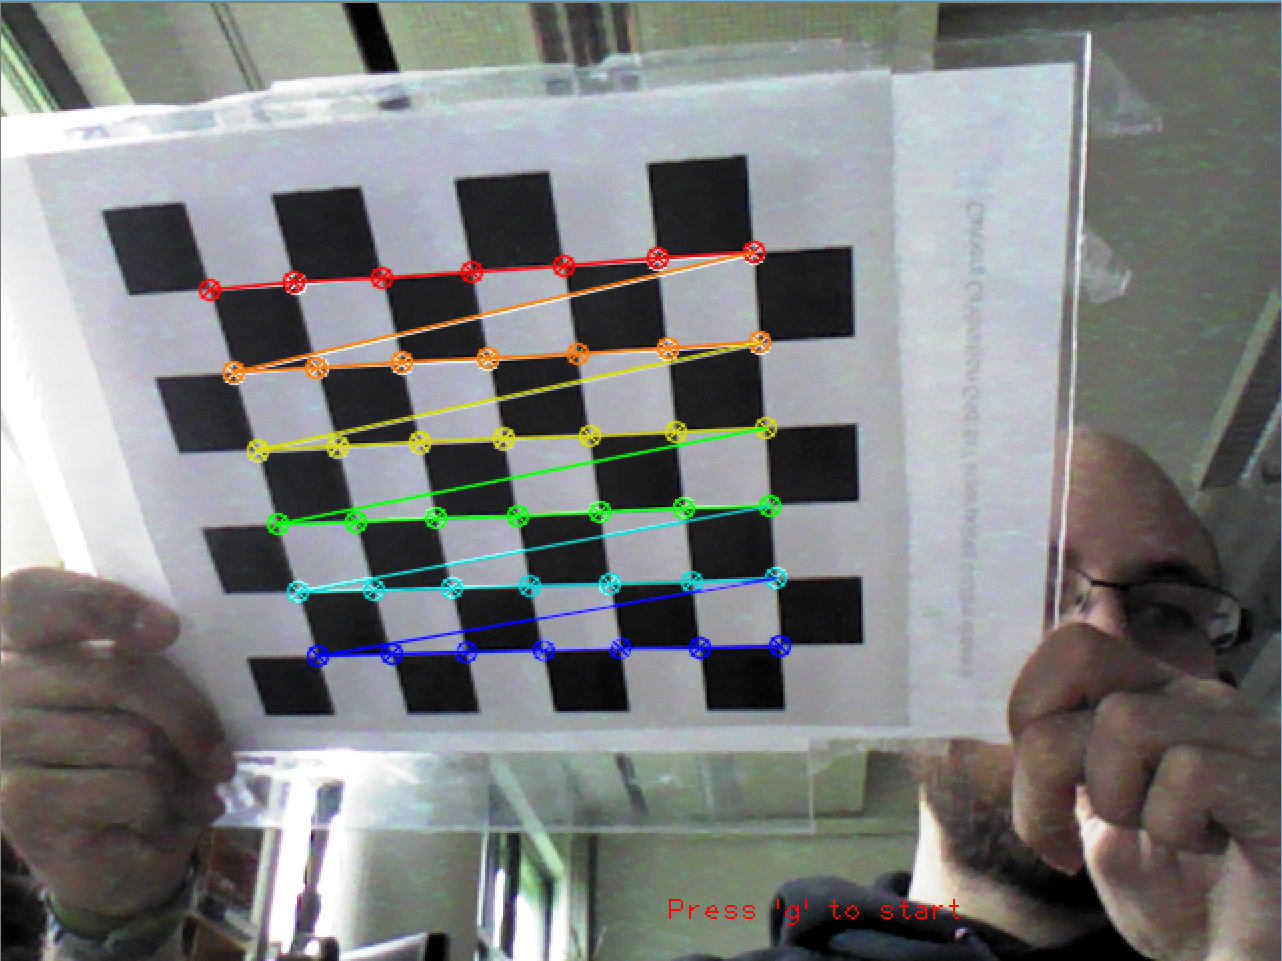
\includegraphics[scale=0.6, angle=0]{Files/Figures/calibration.png}
    \caption[Στιγμιότυπο κατά τη διαδικασία της βαθμονόμησης κάμερας μέσω της OpenCV]{ Στιγμιότυπο κατά τη διαδικασία της βαθμονόμησης κάμερας μέσω της OpenCV}
    \label{fig:calibration_screenshot}
\end{figure}



\section{Δημιουργία Markerboard}


Since the game of chess is a tabletop game that always uses a chessboard as a base for placing the chess pieces on, we considered that using a markerboard would be really similar to the use of a chessboard and the occlusion of the markerboard from the users hand would not affect the rendering of virtual chess pieces during a piece movement. That is why, we created a markerboard which consists of 64 markers in a 8x8 grid, just like a board that is used in chess games, as the main marker of the system. A paper published by the founders of ArUco described the methodology that can be used in order to create speci c marker IDs for the markerboard which will have a high number of bit transitions so that they are less likely to be confused with environment objects. While previous works impose xed dictionaries, the latest version of ArUco library proposes an automatic method for generating a board of marker with the desired number of markers and with the desired number of bits. We used the ArUco samples and created a board of highly reliable markers which corresponds to the size and dimensions of a real chessboard as described by the World Chess Organization.



\section{Αναγνώριση Χειρονομίας Τσιμπήματος}

%wang,popovi
Pinch / Click Detection A robust pinch detector is the basis
of our gestures, and we address it separately from 3D tracking.
Our pinch detection is based on detecting separation of
the tips of the index finger and thumb in at least one of the
two camera images. First, we check for extrema [18] of the
silhouette close to the predicted locations of the index finger
and thumb from our 3D pose estimate. Thumb-index separation
is detected if the geodesic distance between the extrema
is longer than the Euclidean distance. If no separation is detected
in either view, we register a pinch (Figure 12).

%--


The pinch is a basic gesture that can be used to interact on a 3D space rather than a pointing gesture that is usually used on 2D view systems, which is simpler and well performed. On a user-based gesture taxonomy developed [22], [30], several gestures such as ponting, pinch, grab, stretch (using both hands) have been classified according to user experience. The pinch gesture in an AR interaction space is performed several times to imply natural movements and other gestures like selection, shrink/stretch in different axis, rotation, either using one hand or both[30]. Hence, its recognition is fundamental for following basic interactions. On this work, we have implemented a pinch recognition algorithm that triggers a grabbing action to move and release virtual objects in the AR scene based on the hand coordinates exposed from the Leap Motion’s API. The algorithm, Figure 14 runs on a Hand Controller -explained in the next section- which gets the information tracked from the device. Once a hand is recognized, a list of fingers ordered from thumb[0] to pinky[4] are obtained. It consists on identify the thumb fingertip (thumb = finger[0]); calculate a fixed threshold value experimentally based on a proportion of 0.7 times the thumb’s size; from the Fingers list, obtain the fingertip position of each remaining fingers and compare the euclidean distance, equation 3.1 from the thumb to the current finger positions with the threshold value, if the resulting PinchDistance is lower, then a flag is activated, indicating that a pinch has been performed.Afterwards, the grabbing function is performed when the pinch flag is activated. It generates a bounding sphere around the pinch position of the thumb and initializes a vector GrabDistance that will be used to store the difference of distance from the pinch position to the found collided object -this is used to grab only a single object that is closer to the pinch position-; then it identifies each object that collides with the bounding sphere and updates the GrabDistance vector with the difference of the pinch position and the collided object. If the updated distance is less than the GrabDistance of the previous collided object, the object is set as grabbed and a force -a vector calculated from the difference of the pinch position and the position of the grabbed object- is added to the rigid body of the object in order to follow the position of the pinch. When the PinchDistance is higher, the grabbing and pinching flags are disabled. This grabbing function is based on [1] example algorithms.The design is compared with a built-in pinch strength measure from the SDK, the most recent version of the Leap Motion’s SDK provides an automatic measure of the pinch strength value that ranges from [0-1], where 0 corresponds to the open hand with fingers extended and 1 to a full pinch, varying while you move the thumb and other fingers toward each other. On the next chapter 4, the evaluation is explained in more detail


\section{Tαυτοποίηση Συστημάτων Συντεταγμένων}

Coordinate Systems Matching A first step is to consider a unified coordinate system between the AR target and hand tracking sensor. The simplest coordinate systems matching is based on the assumption that our AR marker and sensor are placed on the same origin, when this is not the case, i.e. the sensor and marker are placed in different areas from the camera view perspective, a translation of the Leap Motion’s pose matrix needs to be performed by using the AR marker as a reference. A solution to this, is to use the image target to act as the world center and bring the Leap Motion’s coordinate system by multiplying the inverse pose of our main target (image target) by the pose of the Leap Motion’s target. This creates an offset matrix that can be used to bring points from Leap Motion to image target coordinate system[47]. Nevertheless, for our prototype purpose, it is assumed that the AR marker and sensor are placed in the same origin, where it matches both coordinate systems. This is done, both programmatically, through the game engine and physically where are adjusted in the same origin from a camera view perspective as seen on the Figure.


\section{Απεικόνιση Εικονικών Αντικειμένων} \label{s:rendering}
%σελ 25 jimenez
Although the Unity platform deals with the graphics and integration of libraries for this project, it is necessary to give a deeper review of the process by explaining the target pose calculation and content positioning in the AR framework and the hand controller’s integration. The AR framework exposes a 3x4 Pose Matrix, equation 3.2 that represents the pose of a target with respect to the camera plane. The left 3X3 matrix expresses the rotation matrix, which indicates how the target is rotated while the right column is the translation vector, which is the position of the target as seen from the camera[47], e.g. an identity matrix indicates that the target is parallel to the camera plane (rotation) and a vector (0,0,0) indicates the camera and the target are in the same position.

To position content on the target, the first step is to know the projection matrix -4x4 matrix that projects the scene to the image plane of the camera[49]- that is created with the intrinsic camera calibration parameters, vuforia uses a right handed coordinate system (with the camera origin pointing into the positive z-axis, x-axis to the right and y-axis is downwards) because it is the same coordinate system for targets (just rotated 90 degrees around the x axis: x-axis to the right, y-axis is upwards and z-axis points out of the target-plane; in Unity, z-axis is upwards and y-axis points out of the target)[47]. Once we know the projection matrix we need to set a perspective frustrum from it, where a near and far planes must be set and the size of our trackable -defined in the dataset with feature- should fall within these two planes, Figure 18.
With these requirements in mind, the virtual content (vertices, normals, indices, texture coordinates)
is placed according to the pose matrix calculated at runtime.
The Leap Motion coordinates can be used to move a virtual object, firstly, normalizing and
transforming to suitable coordinates in the interaction box, Figure 13 explained previously.

\section{Χειρισμός Εικονικών Αντικειμένων} \label{s:manipulation}
%ΠΩΣ ΜΕΤΑΚΙΝΟΥΝΤΑΙ ΤΑ ΠΙΟΝΙΑ ΜΕ ΒΑΣΗ ΤΟΝ ΑΛΓΟΡΙΘΜΟ ΜΟΥ
%wang-paris-popovi

-Object translation 
When the user pinches with one hand,
we select the closest object, and translate according to the
pinching hand.


\section{Αντιμετώπιση Απόκρυψης Αντικειμένων} \label{s:occlusion}
%OCCLUSION HANDLING

In this section, the depth estimation of real world is described.
The depth estimation is used to compose the image
of the virtual objects and the image of the real world without
occlusion conflicts. In order to avoid occlusion conflicts, we
need the depth information of only the region onto which
virtual objects are projected. When the positions of virtual
objects are known, the region for depth estimation can be
limited as shown in Figure 4. Therefore, the depth estimation
region of real world can be determined by projecting
a CG object’s bounding box using the model-view matrix
estimated in Section 3.1. The following steps describe a
method of depth estimation of real world.
1. A position of the CG object in the world coordinate
system is transformed into its position in the camera
coordinate system using the estimated model-view matrix
M.
2. A bounding box of the virtual object is projected onto
the left image as shown in Figure 4. A depth estimation
region is obtained as a bounding rectangle of the
projected box. The same process is done for the right
image as well.
3. By adopting the Sobel filter, edges are detected in the
region of depth estimation on the left and right images
4. Stereo matching is performed and the depth value is
computed. Note that only pixels on detected edges in
the left image are matched to those in the right image,
matching window size is 5 x 5 pixels, and similarity
measure is the sum of absolute differences (SAD). In
the same way, the right image as a reference image is
matched to the left image.
5. Matching errors are excluded by considering the consistency
between left-to-right and right-to-left matchings.
The depth values at the pixels between the edges
are interpolated.

By using the estimated model-view matrix and the depth
map of the real world, CG images of virtual objects are
mixed into the image of real world. At this stage, the depth
of real world and each virtual object are compared. When
the real objects are closer to the user’s viewpoint, a transparent
virtual object is drawn at the 3-D position where the
real objects exist. By using a hardware z buffering algorithm,
the virtual objects that are farther than the transparent
objects are not actually drawn on the frame buffer. Therefore
the composed image is looked as if the real objects are
occluding the virtual objects. These rendering steps are illustrated
with examples in Figure 5.
First, only the background image of a real scene is rendered
on the frame buffer as in Figure 5 (a). Z-buffer value
is also set to the farthest value through out the screen. Then,
Z-buffer of the real objects are set to the depth of the real
objects in Figure 5 (c). The regions of real objects are illustrated
with gray levels of depth in Figure 5 (b). Finally, the
virtual objects are rendered by using the model-view matrix
in Figure 5 (d),(e). These steps are applied to both left and right images for obtaining a stereo pair of composite
images.

%-----

For a user to successfully perform tasks in mixed reality environments, a certain level of im- mersion should be provided by the system. In most approaches occlusions are not taken into consideration, so virtual objects are always rendered on top of physical objects. However, to create an immersive and realistic experience, the occlusion between virtual and real objects has to be managed correctly, so that users can look at a scene where virtual content blends with the natural environment. Such an approach allows us to achieve high level of user immersion since the augmented objects occlude the users hands properly; something which is not possible with conventional AR. In OpenGL, when an object is rendered, the depth of a generated pixel (z coordinate) is stored in a buffer, called the z-buffer or depth buffer. This buffer is usually arranged as a two-dimensional array (x-y) with one element for each screen pixel. If another object of the scene must be rendered in the same pixel, the method compares the two depths and overrides the current pixel if the object is closer to the observer. The chosen depth is then saved to the z-buffer, replacing the old one. In the end, the z-buffer will allow the method to correctly reproduce the usual depth perception: a close object hides a farther one.

The main problem when dealing with occlusion is that usually there is no depth information of the real scene. In order to overcome this problem, the depth of the real world from the users viewpoint has to be employed. In the current work, we use the Realsense 3D cameras depth sensor to aid in the process of acquiring the depth map of the environment scene. The Realsense 3D Camera can measure the distance of everything it sees, creating a depth map. This way the depth of every pixel of the depth frame can be estimated. The depth image is basically a 640480 (although it can be smaller) matrix where each pixel value represents the distance from the camera to that point in space (expressed in mm). When a video card renders a virtual scene it computes occlusion from the depth buffer, i.e. the z distance of every object in the virtual scene. Usually when another virtual object must be rendered in the same pixel of the z-buffer, the method compares the 2 depths and overrides the current pixel, if the object is closer to the observer, which in this case is our camera. The trick is to initialize the Z-Buffer of OpenGL with the depth values taken from the Realsense 3D Camera depth image before rendering any 3D virtual object and after rendering the quad which shows the color video stream. By doing so, when the chess pieces are rendered, they will be occluded by what it appears to be real-life objects such as our hand. Its like simulating a render of the entire environment in 3D and using the resulting z-buffer values. So, in order to handle occlusion in our application, we had to map the whole depth image to the color image, transform the values in millimeters to meters and then write to the OpenGLs z-buffer. Before we jump into writing in the z-buffer we need to consider what kind of projection we use (ortho or perspective). So we have to modify the data based on the perspective view that the virtual objects are rendered. In our case virtual objects are drawn using perspective projection. For a perspective projection, the relationship between Z and depth is non-linear. Speci cally, it's of the form

EQUATION


Also we have to bear in mind that points in front of the viewpoint have negative Z coordinates. After applying this transformation to the depth data we can write the data to the z-buffer.Once we write our depth data to the buffer, we can see that virtual object and real objects (such as our hands) blend naturally together.




\section{Ενσωμάτωση Μηχανής Σκακιού}

After the implementation of the pinch gesture detection algorithm, we decided that for our applications purposes, user should be able to play against the computer. This way, a natural sequence of chess events would take place and the application would simulate a real chess game against an opponent, something that would help with the evaluation of the system. In order for the user to be able to play against a computer, normally, we need to implement arti cial intelligence algorithms so that our program could think the next move based on the past moves made by the user. However the implementation of these algorithms for our chess game was out of the scope of this thesis and a simple way for AI functionality integration had to be investigated. This is where the chess engines emerge. A chess engine is a computer program that that receives a board position as input, analyzes the position of chess pieces and calculates the best move based on that board within a given amount of possible effort (in most cases a time limit). The chess engine estimates the next moves, but typically does not interact directly with the user. Most chess engines do not have their own graphical user interface (GUI) but are rather console applications that communicate with a GUI via a standard protocol. This allows the user to play against multiple engines without learning a new user interface for each, and allows different engines to play against each other. The GUI, in this case, is our application so far. What we need is a way to connect it with the chess engine properly. Nowadays, the most used way of communication with a chess engine is the Universal Chess Interface (UCI) Protocol. The Universal Chess Interface (UCI) is an open communication protocol that enables a chess program's engine to communicate with its user interface through a set of speci c commands. In order to integrate a chess engine to the augmented reality chess game, we need to exchange commands(strings) with a chess engine. A chess engine receives commands via standard input from an application and outputs its responses to standard output. So it has no graphical user interface, no mouse input, no pictures, just a plain console window, it is nothing more than an executable. To communicate with the engines executable, we decided to use a feature provided by Qt, through a class named QProcess which allows to start an executable le and easily read and write string commands from and to it. The interaction with the engine starts with a uci command that tells the engine to identify itself. It then receives commands that may change the values of options and the way output is presented by the engine. Afterwards, the engine takes as an input from our application the users completed move, and outputs the next best move for the enemy pieces. The chess engine is told to spend a speci c amount of time to search for a best move. It starts its search and considers the best move before the time limit expires. For our application we considered that the time limit should be really small(40ms) so that we can get immediate feedback from our program. Usually, chess engines dont have the ability to know whether or not a move command by the user is a valid one or not, based on the pieces type and the state of the board. However, we used the iCE Engine[link] which stores the possible moves for every chess piece and when an invalid move is taken as an input from the user, it returns the string Invalid chess move. This feature really helped us in changing the architecture of our code logic and makes it even easier for the user not to execute a wrong move at all. What is more, the engine we used can output the outcome of the game, so that our program can detect if the user won or lost the game. So we implemented the basic functionality to send and receive strings to and from the engine and according to these strings the correct actions can be taken in our program.










 